\documentclass[]{article}
\usepackage{lmodern}
\usepackage{amssymb,amsmath}
\usepackage{ifxetex,ifluatex}
\usepackage{fixltx2e} % provides \textsubscript
\ifnum 0\ifxetex 1\fi\ifluatex 1\fi=0 % if pdftex
  \usepackage[T1]{fontenc}
  \usepackage[utf8]{inputenc}
\else % if luatex or xelatex
  \ifxetex
    \usepackage{mathspec}
  \else
    \usepackage{fontspec}
  \fi
  \defaultfontfeatures{Ligatures=TeX,Scale=MatchLowercase}
\fi
% use upquote if available, for straight quotes in verbatim environments
\IfFileExists{upquote.sty}{\usepackage{upquote}}{}
% use microtype if available
\IfFileExists{microtype.sty}{%
\usepackage{microtype}
\UseMicrotypeSet[protrusion]{basicmath} % disable protrusion for tt fonts
}{}
\usepackage[margin=2.54cm]{geometry}
\usepackage{hyperref}
\hypersetup{unicode=true,
            pdftitle={Assignment 3: Data Exploration},
            pdfauthor={Xin Wang},
            pdfborder={0 0 0},
            breaklinks=true}
\urlstyle{same}  % don't use monospace font for urls
\usepackage{color}
\usepackage{fancyvrb}
\newcommand{\VerbBar}{|}
\newcommand{\VERB}{\Verb[commandchars=\\\{\}]}
\DefineVerbatimEnvironment{Highlighting}{Verbatim}{commandchars=\\\{\}}
% Add ',fontsize=\small' for more characters per line
\usepackage{framed}
\definecolor{shadecolor}{RGB}{248,248,248}
\newenvironment{Shaded}{\begin{snugshade}}{\end{snugshade}}
\newcommand{\KeywordTok}[1]{\textcolor[rgb]{0.13,0.29,0.53}{\textbf{#1}}}
\newcommand{\DataTypeTok}[1]{\textcolor[rgb]{0.13,0.29,0.53}{#1}}
\newcommand{\DecValTok}[1]{\textcolor[rgb]{0.00,0.00,0.81}{#1}}
\newcommand{\BaseNTok}[1]{\textcolor[rgb]{0.00,0.00,0.81}{#1}}
\newcommand{\FloatTok}[1]{\textcolor[rgb]{0.00,0.00,0.81}{#1}}
\newcommand{\ConstantTok}[1]{\textcolor[rgb]{0.00,0.00,0.00}{#1}}
\newcommand{\CharTok}[1]{\textcolor[rgb]{0.31,0.60,0.02}{#1}}
\newcommand{\SpecialCharTok}[1]{\textcolor[rgb]{0.00,0.00,0.00}{#1}}
\newcommand{\StringTok}[1]{\textcolor[rgb]{0.31,0.60,0.02}{#1}}
\newcommand{\VerbatimStringTok}[1]{\textcolor[rgb]{0.31,0.60,0.02}{#1}}
\newcommand{\SpecialStringTok}[1]{\textcolor[rgb]{0.31,0.60,0.02}{#1}}
\newcommand{\ImportTok}[1]{#1}
\newcommand{\CommentTok}[1]{\textcolor[rgb]{0.56,0.35,0.01}{\textit{#1}}}
\newcommand{\DocumentationTok}[1]{\textcolor[rgb]{0.56,0.35,0.01}{\textbf{\textit{#1}}}}
\newcommand{\AnnotationTok}[1]{\textcolor[rgb]{0.56,0.35,0.01}{\textbf{\textit{#1}}}}
\newcommand{\CommentVarTok}[1]{\textcolor[rgb]{0.56,0.35,0.01}{\textbf{\textit{#1}}}}
\newcommand{\OtherTok}[1]{\textcolor[rgb]{0.56,0.35,0.01}{#1}}
\newcommand{\FunctionTok}[1]{\textcolor[rgb]{0.00,0.00,0.00}{#1}}
\newcommand{\VariableTok}[1]{\textcolor[rgb]{0.00,0.00,0.00}{#1}}
\newcommand{\ControlFlowTok}[1]{\textcolor[rgb]{0.13,0.29,0.53}{\textbf{#1}}}
\newcommand{\OperatorTok}[1]{\textcolor[rgb]{0.81,0.36,0.00}{\textbf{#1}}}
\newcommand{\BuiltInTok}[1]{#1}
\newcommand{\ExtensionTok}[1]{#1}
\newcommand{\PreprocessorTok}[1]{\textcolor[rgb]{0.56,0.35,0.01}{\textit{#1}}}
\newcommand{\AttributeTok}[1]{\textcolor[rgb]{0.77,0.63,0.00}{#1}}
\newcommand{\RegionMarkerTok}[1]{#1}
\newcommand{\InformationTok}[1]{\textcolor[rgb]{0.56,0.35,0.01}{\textbf{\textit{#1}}}}
\newcommand{\WarningTok}[1]{\textcolor[rgb]{0.56,0.35,0.01}{\textbf{\textit{#1}}}}
\newcommand{\AlertTok}[1]{\textcolor[rgb]{0.94,0.16,0.16}{#1}}
\newcommand{\ErrorTok}[1]{\textcolor[rgb]{0.64,0.00,0.00}{\textbf{#1}}}
\newcommand{\NormalTok}[1]{#1}
\usepackage{graphicx,grffile}
\makeatletter
\def\maxwidth{\ifdim\Gin@nat@width>\linewidth\linewidth\else\Gin@nat@width\fi}
\def\maxheight{\ifdim\Gin@nat@height>\textheight\textheight\else\Gin@nat@height\fi}
\makeatother
% Scale images if necessary, so that they will not overflow the page
% margins by default, and it is still possible to overwrite the defaults
% using explicit options in \includegraphics[width, height, ...]{}
\setkeys{Gin}{width=\maxwidth,height=\maxheight,keepaspectratio}
\IfFileExists{parskip.sty}{%
\usepackage{parskip}
}{% else
\setlength{\parindent}{0pt}
\setlength{\parskip}{6pt plus 2pt minus 1pt}
}
\setlength{\emergencystretch}{3em}  % prevent overfull lines
\providecommand{\tightlist}{%
  \setlength{\itemsep}{0pt}\setlength{\parskip}{0pt}}
\setcounter{secnumdepth}{0}
% Redefines (sub)paragraphs to behave more like sections
\ifx\paragraph\undefined\else
\let\oldparagraph\paragraph
\renewcommand{\paragraph}[1]{\oldparagraph{#1}\mbox{}}
\fi
\ifx\subparagraph\undefined\else
\let\oldsubparagraph\subparagraph
\renewcommand{\subparagraph}[1]{\oldsubparagraph{#1}\mbox{}}
\fi

%%% Use protect on footnotes to avoid problems with footnotes in titles
\let\rmarkdownfootnote\footnote%
\def\footnote{\protect\rmarkdownfootnote}

%%% Change title format to be more compact
\usepackage{titling}

% Create subtitle command for use in maketitle
\newcommand{\subtitle}[1]{
  \posttitle{
    \begin{center}\large#1\end{center}
    }
}

\setlength{\droptitle}{-2em}

  \title{Assignment 3: Data Exploration}
    \pretitle{\vspace{\droptitle}\centering\huge}
  \posttitle{\par}
    \author{Xin Wang}
    \preauthor{\centering\large\emph}
  \postauthor{\par}
    \date{}
    \predate{}\postdate{}
  

\begin{document}
\maketitle

\subsection{OVERVIEW}\label{overview}

This exercise accompanies the lessons in Environmental Data Analytics
(ENV872L) on data exploration.

\subsection{Directions}\label{directions}

\begin{enumerate}
\def\labelenumi{\arabic{enumi}.}
\tightlist
\item
  Change ``Student Name'' on line 3 (above) with your name.
\item
  Use the lesson as a guide. It contains code that can be modified to
  complete the assignment.
\item
  Work through the steps, \textbf{creating code and output} that fulfill
  each instruction.
\item
  Be sure to \textbf{answer the questions} in this assignment document.
  Space for your answers is provided in this document and is indicated
  by the ``\textgreater{}'' character. If you need a second paragraph be
  sure to start the first line with ``\textgreater{}''. You should
  notice that the answer is highlighted in green by RStudio.
\item
  When you have completed the assignment, \textbf{Knit} the text and
  code into a single PDF file. You will need to have the correct
  software installed to do this (see Software Installation Guide) Press
  the \texttt{Knit} button in the RStudio scripting panel. This will
  save the PDF output in your Assignments folder.
\item
  After Knitting, please submit the completed exercise (PDF file) to the
  dropbox in Sakai. Please add your last name into the file name (e.g.,
  ``Salk\_A02\_DataExploration.pdf'') prior to submission.
\end{enumerate}

The completed exercise is due on Thursday, 31 January, 2019 before class
begins.

\subsection{1) Set up your R session}\label{set-up-your-r-session}

Check your working directory, load necessary packages (tidyverse), and
upload the North Temperate Lakes long term monitoring dataset for the
light, temperature, and oxygen data for three lakes (file name:
NTL-LTER\_Lake\_ChemistryPhysics\_Raw.csv). Type your code into the R
chunk below.

\begin{Shaded}
\begin{Highlighting}[]
\KeywordTok{getwd}\NormalTok{()}
\end{Highlighting}
\end{Shaded}

\begin{verbatim}
## [1] "Y:/19spring/872/Environmental_Data_Analytics/Assignments"
\end{verbatim}

\begin{Shaded}
\begin{Highlighting}[]
\KeywordTok{library}\NormalTok{(tidyverse)}
\end{Highlighting}
\end{Shaded}

\begin{verbatim}
## Warning: package 'tidyverse' was built under R version 3.5.2
\end{verbatim}

\begin{verbatim}
## -- Attaching packages -------------------------------------------------------------------------------- tidyverse 1.2.1 --
\end{verbatim}

\begin{verbatim}
## v ggplot2 3.1.0     v purrr   0.2.5
## v tibble  1.4.2     v dplyr   0.7.8
## v tidyr   0.8.2     v stringr 1.3.1
## v readr   1.3.1     v forcats 0.3.0
\end{verbatim}

\begin{verbatim}
## Warning: package 'ggplot2' was built under R version 3.5.2
\end{verbatim}

\begin{verbatim}
## Warning: package 'tibble' was built under R version 3.5.2
\end{verbatim}

\begin{verbatim}
## Warning: package 'tidyr' was built under R version 3.5.2
\end{verbatim}

\begin{verbatim}
## Warning: package 'readr' was built under R version 3.5.2
\end{verbatim}

\begin{verbatim}
## Warning: package 'purrr' was built under R version 3.5.2
\end{verbatim}

\begin{verbatim}
## Warning: package 'dplyr' was built under R version 3.5.2
\end{verbatim}

\begin{verbatim}
## Warning: package 'stringr' was built under R version 3.5.2
\end{verbatim}

\begin{verbatim}
## Warning: package 'forcats' was built under R version 3.5.2
\end{verbatim}

\begin{verbatim}
## -- Conflicts ----------------------------------------------------------------------------------- tidyverse_conflicts() --
## x dplyr::filter() masks stats::filter()
## x dplyr::lag()    masks stats::lag()
\end{verbatim}

\begin{Shaded}
\begin{Highlighting}[]
\NormalTok{NTL.dat <-}\StringTok{ }\KeywordTok{read.csv}\NormalTok{(}\StringTok{"../Data/Raw/NTL-LTER_Lake_ChemistryPhysics_Raw.csv"}\NormalTok{)}
\end{Highlighting}
\end{Shaded}

\subsection{2) Learn about your system}\label{learn-about-your-system}

Read about your dataset in the NTL-LTER README file. What are three
salient pieces of information you gained from reading this file?

\begin{quote}
ANSWER: The source of the data (LTER project), its time span (1984-2016)
and collection methodology (location, time, sampling method, etc.).
\end{quote}

\subsection{3) Obtain basic summaries of your
data}\label{obtain-basic-summaries-of-your-data}

Write R commands to display the following information:

\begin{enumerate}
\def\labelenumi{\arabic{enumi}.}
\tightlist
\item
  dimensions of the dataset
\item
  class of the dataset
\item
  first 8 rows of the dataset
\item
  class of the variables lakename, sampledate, depth, and temperature
\item
  summary of lakename, depth, and temperature
\end{enumerate}

\begin{Shaded}
\begin{Highlighting}[]
\CommentTok{# 1}
\KeywordTok{dim}\NormalTok{(NTL.dat)}
\end{Highlighting}
\end{Shaded}

\begin{verbatim}
## [1] 38614    11
\end{verbatim}

\begin{Shaded}
\begin{Highlighting}[]
\CommentTok{# 2}
\KeywordTok{class}\NormalTok{(NTL.dat)}
\end{Highlighting}
\end{Shaded}

\begin{verbatim}
## [1] "data.frame"
\end{verbatim}

\begin{Shaded}
\begin{Highlighting}[]
\CommentTok{# 3}
\KeywordTok{head}\NormalTok{(NTL.dat,}\DecValTok{8}\NormalTok{)}
\end{Highlighting}
\end{Shaded}

\begin{verbatim}
##   lakeid  lakename year4 daynum sampledate depth temperature_C
## 1      L Paul Lake  1984    148    5/27/84  0.00          14.5
## 2      L Paul Lake  1984    148    5/27/84  0.25            NA
## 3      L Paul Lake  1984    148    5/27/84  0.50            NA
## 4      L Paul Lake  1984    148    5/27/84  0.75            NA
## 5      L Paul Lake  1984    148    5/27/84  1.00          14.5
## 6      L Paul Lake  1984    148    5/27/84  1.50            NA
## 7      L Paul Lake  1984    148    5/27/84  2.00          14.2
## 8      L Paul Lake  1984    148    5/27/84  3.00          11.0
##   dissolvedOxygen irradianceWater irradianceDeck comments
## 1             9.5            1750           1620     <NA>
## 2              NA            1550           1620     <NA>
## 3              NA            1150           1620     <NA>
## 4              NA             975           1620     <NA>
## 5             8.8             870           1620     <NA>
## 6              NA             610           1620     <NA>
## 7             8.6             420           1620     <NA>
## 8            11.5             220           1620     <NA>
\end{verbatim}

\begin{Shaded}
\begin{Highlighting}[]
\CommentTok{# 4}
\KeywordTok{attach}\NormalTok{(NTL.dat)}
\KeywordTok{class}\NormalTok{(lakename)}
\end{Highlighting}
\end{Shaded}

\begin{verbatim}
## [1] "factor"
\end{verbatim}

\begin{Shaded}
\begin{Highlighting}[]
\KeywordTok{class}\NormalTok{(sampledate)}
\end{Highlighting}
\end{Shaded}

\begin{verbatim}
## [1] "factor"
\end{verbatim}

\begin{Shaded}
\begin{Highlighting}[]
\KeywordTok{class}\NormalTok{(depth)}
\end{Highlighting}
\end{Shaded}

\begin{verbatim}
## [1] "numeric"
\end{verbatim}

\begin{Shaded}
\begin{Highlighting}[]
\KeywordTok{class}\NormalTok{(temperature_C)}
\end{Highlighting}
\end{Shaded}

\begin{verbatim}
## [1] "numeric"
\end{verbatim}

\begin{Shaded}
\begin{Highlighting}[]
\CommentTok{# 5}
\KeywordTok{summary}\NormalTok{(lakename)}
\end{Highlighting}
\end{Shaded}

\begin{verbatim}
## Central Long Lake     Crampton Lake    East Long Lake  Hummingbird Lake 
##               539              1234              3905               430 
##         Paul Lake        Peter Lake      Tuesday Lake         Ward Lake 
##             10325             11288              6107               598 
##    West Long Lake 
##              4188
\end{verbatim}

\begin{Shaded}
\begin{Highlighting}[]
\KeywordTok{summary}\NormalTok{(depth)}
\end{Highlighting}
\end{Shaded}

\begin{verbatim}
##    Min. 1st Qu.  Median    Mean 3rd Qu.    Max. 
##    0.00    1.50    4.00    4.39    6.50   20.00
\end{verbatim}

\begin{Shaded}
\begin{Highlighting}[]
\KeywordTok{summary}\NormalTok{(temperature_C)}
\end{Highlighting}
\end{Shaded}

\begin{verbatim}
##    Min. 1st Qu.  Median    Mean 3rd Qu.    Max.    NA's 
##    0.30    5.30    9.30   11.81   18.70   34.10    3858
\end{verbatim}

\begin{Shaded}
\begin{Highlighting}[]
\KeywordTok{detach}\NormalTok{(NTL.dat)}
\end{Highlighting}
\end{Shaded}

Change sampledate to class = date. After doing this, write an R command
to display that the class of sammpledate is indeed date. Write another R
command to show the first 10 rows of the date column.

\begin{Shaded}
\begin{Highlighting}[]
\NormalTok{NTL.dat}\OperatorTok{$}\NormalTok{sampledate <-}\StringTok{ }\KeywordTok{as.Date}\NormalTok{(NTL.dat}\OperatorTok{$}\NormalTok{sampledate,}\DataTypeTok{format =} \StringTok{"%m/%d/%y"}\NormalTok{)}
\KeywordTok{class}\NormalTok{(NTL.dat}\OperatorTok{$}\NormalTok{sampledate)}
\end{Highlighting}
\end{Shaded}

\begin{verbatim}
## [1] "Date"
\end{verbatim}

\begin{Shaded}
\begin{Highlighting}[]
\KeywordTok{head}\NormalTok{(NTL.dat}\OperatorTok{$}\NormalTok{sampledate,}\DecValTok{10}\NormalTok{)}
\end{Highlighting}
\end{Shaded}

\begin{verbatim}
##  [1] "1984-05-27" "1984-05-27" "1984-05-27" "1984-05-27" "1984-05-27"
##  [6] "1984-05-27" "1984-05-27" "1984-05-27" "1984-05-27" "1984-05-27"
\end{verbatim}

Question: Do you want to remove NAs from this dataset? Why or why not?

\begin{quote}
ANSWER: No, because each row represents the measurement at a unique
depth for a certain lake on a certain day. There's no repititions, so
each row matters, even if it has NAs.
\end{quote}

\subsection{4) Explore your data
graphically}\label{explore-your-data-graphically}

Write R commands to display graphs depicting:

\begin{enumerate}
\def\labelenumi{\arabic{enumi}.}
\tightlist
\item
  Bar chart of temperature counts for each lake
\item
  Histogram of count distributions of temperature (all temp measurements
  together)
\item
  Change histogram from 2 to have a different number or width of bins
\item
  Frequency polygon of temperature for each lake. Choose different
  colors for each lake.
\item
  Boxplot of temperature for each lake
\item
  Boxplot of temperature based on depth, with depth divided into 0.25 m
  increments
\item
  Scatterplot of temperature by depth
\end{enumerate}

\begin{Shaded}
\begin{Highlighting}[]
\CommentTok{# 1}
\KeywordTok{attach}\NormalTok{(NTL.dat)}
\KeywordTok{ggplot}\NormalTok{(NTL.dat,}\KeywordTok{aes}\NormalTok{(}\DataTypeTok{x =}\NormalTok{ lakeid)) }\OperatorTok{+}
\StringTok{  }\KeywordTok{geom_bar}\NormalTok{()}
\end{Highlighting}
\end{Shaded}

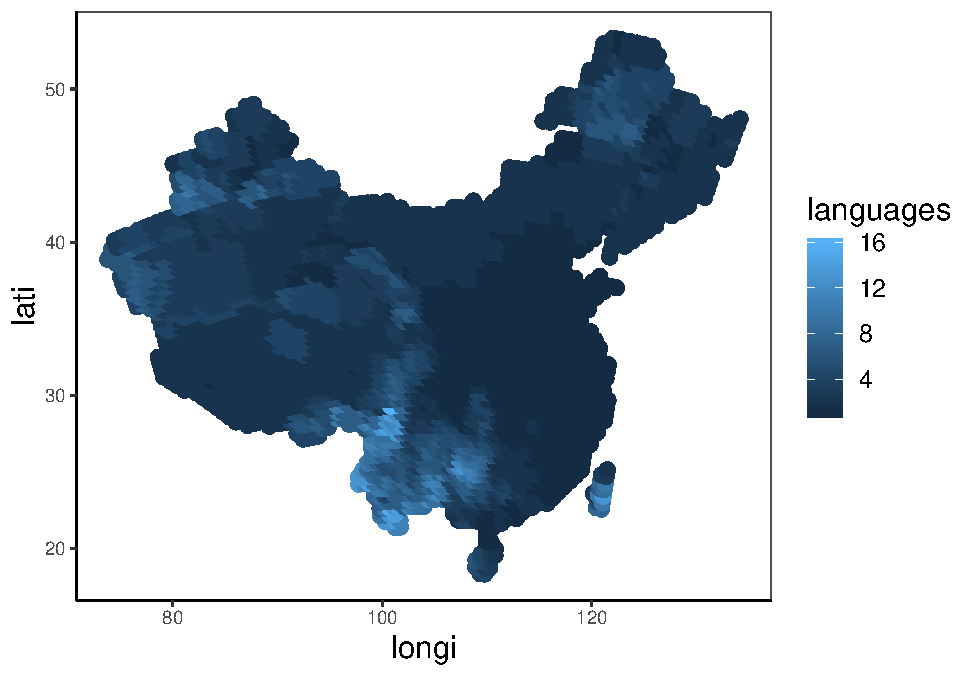
\includegraphics{A03_DataExploration_files/figure-latex/unnamed-chunk-4-1.pdf}

\begin{Shaded}
\begin{Highlighting}[]
\CommentTok{# 2}
\KeywordTok{ggplot}\NormalTok{(NTL.dat) }\OperatorTok{+}
\StringTok{  }\KeywordTok{geom_histogram}\NormalTok{(}\KeywordTok{aes}\NormalTok{(}\DataTypeTok{x =}\NormalTok{ temperature_C))}
\end{Highlighting}
\end{Shaded}

\begin{verbatim}
## `stat_bin()` using `bins = 30`. Pick better value with `binwidth`.
\end{verbatim}

\begin{verbatim}
## Warning: Removed 3858 rows containing non-finite values (stat_bin).
\end{verbatim}

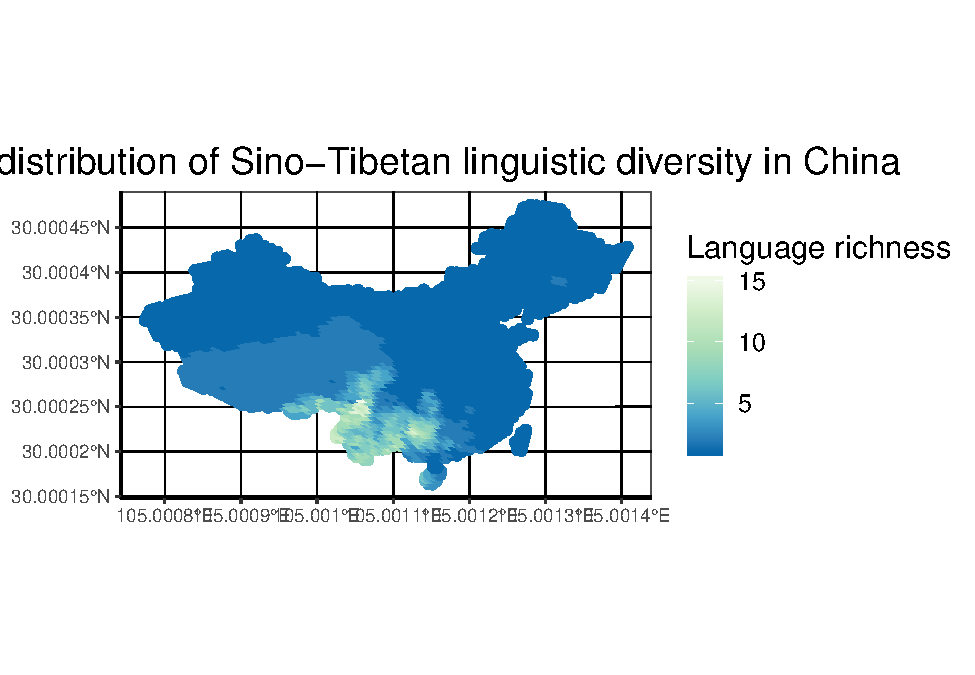
\includegraphics{A03_DataExploration_files/figure-latex/unnamed-chunk-4-2.pdf}

\begin{Shaded}
\begin{Highlighting}[]
\CommentTok{# 3}
\KeywordTok{ggplot}\NormalTok{(NTL.dat) }\OperatorTok{+}
\StringTok{  }\KeywordTok{geom_histogram}\NormalTok{(}\KeywordTok{aes}\NormalTok{(}\DataTypeTok{x =}\NormalTok{ temperature_C),}\DataTypeTok{binwidth =} \FloatTok{0.5}\NormalTok{)}
\end{Highlighting}
\end{Shaded}

\begin{verbatim}
## Warning: Removed 3858 rows containing non-finite values (stat_bin).
\end{verbatim}

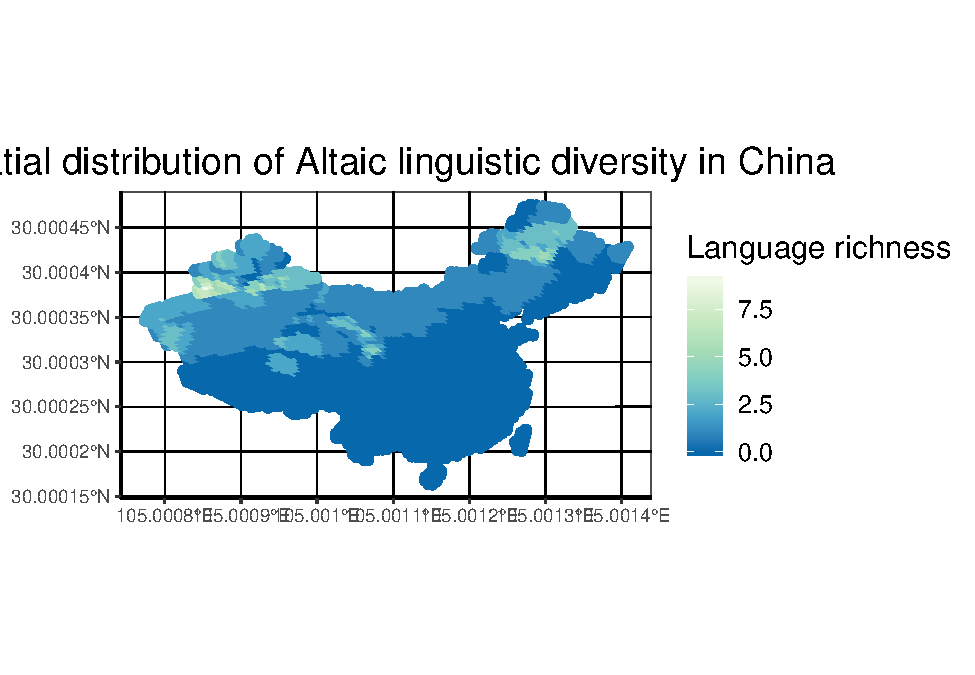
\includegraphics{A03_DataExploration_files/figure-latex/unnamed-chunk-4-3.pdf}

\begin{Shaded}
\begin{Highlighting}[]
\CommentTok{# 4}
\KeywordTok{ggplot}\NormalTok{(NTL.dat) }\OperatorTok{+}
\StringTok{  }\KeywordTok{geom_freqpoly}\NormalTok{(}\KeywordTok{aes}\NormalTok{(}\DataTypeTok{x =}\NormalTok{ temperature_C, }\DataTypeTok{color =}\NormalTok{ lakeid))}
\end{Highlighting}
\end{Shaded}

\begin{verbatim}
## `stat_bin()` using `bins = 30`. Pick better value with `binwidth`.
\end{verbatim}

\begin{verbatim}
## Warning: Removed 3858 rows containing non-finite values (stat_bin).
\end{verbatim}

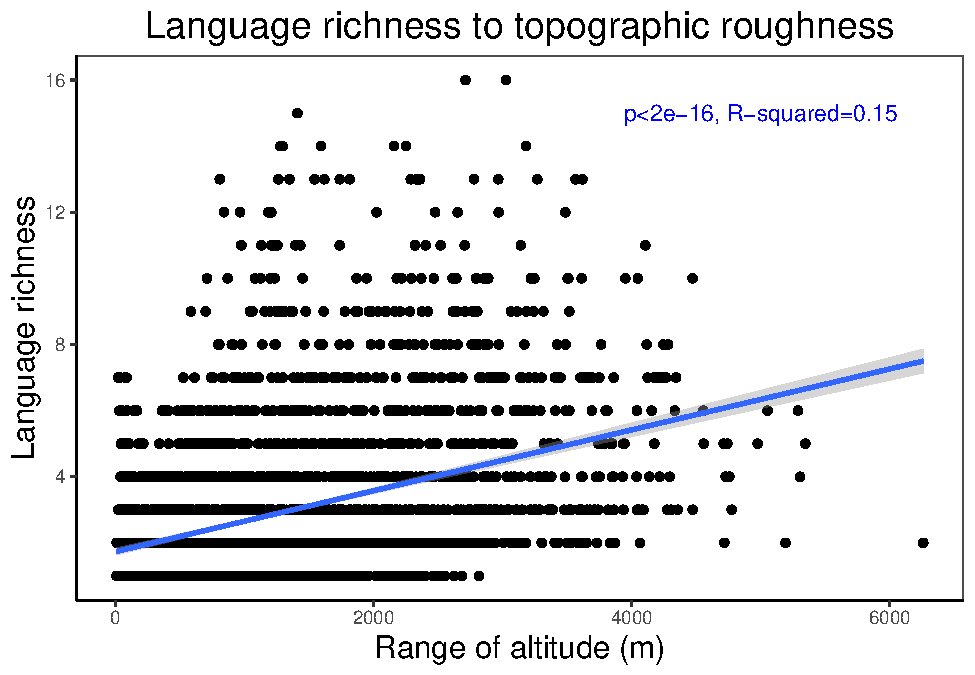
\includegraphics{A03_DataExploration_files/figure-latex/unnamed-chunk-4-4.pdf}

\begin{Shaded}
\begin{Highlighting}[]
\CommentTok{# 5}
\KeywordTok{ggplot}\NormalTok{(NTL.dat) }\OperatorTok{+}
\StringTok{  }\KeywordTok{geom_boxplot}\NormalTok{(}\KeywordTok{aes}\NormalTok{(}\DataTypeTok{x =}\NormalTok{ lakeid,}\DataTypeTok{y =}\NormalTok{ temperature_C))}
\end{Highlighting}
\end{Shaded}

\begin{verbatim}
## Warning: Removed 3858 rows containing non-finite values (stat_boxplot).
\end{verbatim}

\includegraphics{A03_DataExploration_files/figure-latex/unnamed-chunk-4-5.pdf}

\begin{Shaded}
\begin{Highlighting}[]
\CommentTok{# 6}
\KeywordTok{ggplot}\NormalTok{(NTL.dat) }\OperatorTok{+}
\StringTok{  }\KeywordTok{geom_boxplot}\NormalTok{(}\KeywordTok{aes}\NormalTok{(}\DataTypeTok{x =}\NormalTok{ depth, }\DataTypeTok{y =}\NormalTok{ temperature_C, }\DataTypeTok{group =} \KeywordTok{cut_width}\NormalTok{(depth, }\FloatTok{0.25}\NormalTok{)))}
\end{Highlighting}
\end{Shaded}

\begin{verbatim}
## Warning: Removed 3858 rows containing non-finite values (stat_boxplot).
\end{verbatim}

\includegraphics{A03_DataExploration_files/figure-latex/unnamed-chunk-4-6.pdf}

\begin{Shaded}
\begin{Highlighting}[]
\CommentTok{# 7 }
\KeywordTok{ggplot}\NormalTok{(NTL.dat) }\OperatorTok{+}
\StringTok{  }\KeywordTok{geom_point}\NormalTok{(}\KeywordTok{aes}\NormalTok{(}\DataTypeTok{x =}\NormalTok{ depth, }\DataTypeTok{y =}\NormalTok{ temperature_C))}
\end{Highlighting}
\end{Shaded}

\begin{verbatim}
## Warning: Removed 3858 rows containing missing values (geom_point).
\end{verbatim}

\includegraphics{A03_DataExploration_files/figure-latex/unnamed-chunk-4-7.pdf}

\begin{Shaded}
\begin{Highlighting}[]
\KeywordTok{detach}\NormalTok{(NTL.dat)}
\end{Highlighting}
\end{Shaded}

\subsection{5) Form questions for further data
analysis}\label{form-questions-for-further-data-analysis}

What did you find out about your data from the basic summaries and
graphs you made? Describe in 4-6 sentences.

\begin{quote}
ANSWER: There are totally 9 lakes investigated for the project, with
Paul Lake and Peter Lake the most samples. Sampling depth ranges from 0
to 20m, but most samples are collected in water shallower than 10m. The
frequency distribution of temperature among the samples has two peaks,
one around 5 degree celcius and the other around 22 degree celcius.
Generally, water temperature decreases as depth increases, but remains
steady in water deeper than 10m.
\end{quote}

What are 3 further questions you might ask as you move forward with
analysis of this dataset?

\begin{quote}
ANSWER 1: How does dissolved oxygen change with depth?
\end{quote}

\begin{quote}
ANSWER 2: For the physical and chemical variables, is there significant
difference among different lakes?
\end{quote}

\begin{quote}
ANSWER 3: How do the physical and chemical variables of the lakes change
with time?
\end{quote}


\end{document}
